%!TEX root = ../main.tex
Now, let us consider the \gls{sp} $y(t)$ obtained as output of an asymptotically stable digital filter $F(z)$ fed by a \gls{ssp} $v(t)$ as input, but with a generic initialization (not steady-state output).

\begin{figure}[htpb]
	\centering
	\begin{tikzpicture}
		% place nodes
		\node [block] (f) at (0,0) {$F(z)$};

		% connect nodes
		\draw [stealth-] (f.west) -- ++(-2,0) node[midway,above] {$v(t)$};
		\draw [-stealth] (f.east) -- ++(2,0)  node[midway,above] {$y(t)$};
	\end{tikzpicture}
\end{figure}
\FloatBarrier

\begin{theorem}
	There is just one stationary output which corresponds to the steady-state solution. However, if $F(z)$ is asymptotically stable, then all possible outputs obtained for different initialization of the digital filter $F(z)$ tends asymptotically (as $t \rightarrow \infty$) to the steady-state solution, i.e. to the stationary output.
\end{theorem}

\fg{0.7}{steady-state}

\section{Weak (wide-sense) characterization of AR, ARMA processes}
Our goal now is to consider AR and ARMA processes and compute their mean $m_y$ and covariance function $\gamma_y(\tau)$.

%Since the steady-state solution is an MA($\infty$) process we could use such results but are too diffucult

We'll rely on the recursive equation characterizing such processes.

\subsection{AR processes}

Let us consider the AR($1$) (or equivalently ARMA($1,0$)) process generated according to:
\begin{align*}
	y(t)=a \cdot y(t-1)+e(t) \quad \text{where} \quad e(t) \sim \WN(0, \lambda^{2})
\end{align*}

Operatorial representation for $y(t)$:

\begin{align*}
	y(t)&=z^{-1} a y(t)+e(t) \\
	\left(1-z^{-1} a\right) y(t)&=e(t) \\
	y(t)&=\frac{1}{1-z^{-1} a} e(t)
\end{align*}

The transfer function with positive powers (to identify zeros and poles) is $y(t)=\frac{z}{z-a} e(t) \quad$.

There is just one pole: $z=a .$

The process generating system is asymptotically stable if $|a| <1$. 

Since $e(t)$ is a \gls{ssp} (by definition of \gls{wn}), when $|a| <1$ the steady-state output process $y(t)$ is a \gls{ssp}.

\textbf{Mean.}
Start from the time-domain representation and apply expectation to both sides:
\[
	\E[y(t)]=\E[a \cdot y(t-1)+e(t)] \implies \E[y(t)]=a \cdot \E[y(t-1)]+\E[e(t)]
\]
Thanks to stationarity $\E[y(t)]=\E[y(t-1)]=m_{y}$, so that $m_{y}=a \cdot m_{y}+m_{e}$.
Then:
$$
m_{e}=0 \implies  m_{y}=0
$$
\textbf{Variance.}
Let us compute
\[
	\gamma_{y}(0)=\E\left[\left(y(t)-m_{y}\right)^{2}\right]
\]
Remember that $m_{y}=0$. Start from $y(t)=a \cdot y(t-1)+e(t)$, take the square and apply operator $\E[\cdot]$ to both side:
\begin{align*}
	\gamma_{y}(0)&=\E\left[(y(t))^{2}\right]\\
	&=\E\left[(a \cdot y(t-1)+e(t))^{2}\right]\\
	&=a^{2} \E\left[y(t-1)^{2}\right]+\E\left[e(t)^{2}\right]+2 a \E[y(t-1) e(t)]\\
\end{align*}
Mid-term evaluation:
\[
	2 a \E[y(t-1) e(t)]=0,
\]
indeed, by using the MA($\infty$) representation for $y(t-1)$ (AR process):
$$
y(t-1)=e(t-1)+a \cdot e(t-2)+a^{2} \cdot e(t-3)+a^{3} \cdot e(t-4)+\cdots
$$
we have that:
\[
	\E[e(t) y(t-1)]=\E\left[e(t) \cdot\left(e(t-1)+a \cdot e(t-2)+a^{2} \cdot e(t-3)+a^{3} \cdot e(t-4)+\cdots\right)\right]=0
\]
(all products give null contribution thanks to the whiteness property).


$\E\left[(y(t-1))^{2}\right]=\gamma_{y}(0)$

$\E\left[(e(t))^{2}\right]=\lambda^{2}$

Hence,
\[
	\gamma_{y}(0)=a^{2} \gamma_{y}(0)+\lambda^{2} \implies \gamma_{y}(0)=\frac{\lambda^{2}}{1-a^{2}}
\]
\textbf{Covariance.}
Remember that $m_{y}=0$ and substitute $y(t)=a \cdot y(t-1)+e(t)$,
\begin{align*}
	\gamma_{y}(1)&=\E\left[\left(y(t)-m_{y}\right) \cdot\left(y(t-1)-m_{y}\right)\right]\\
	&=\E[y(t) y(t-1)]\\
	&=\E[(a \cdot y(t-1)+e(t))y(t-1)]\\
	&=a \cdot \E\left[(y(t-1))^{2}\right]+\E[e(t) y(t-1)]
\end{align*}

We already know that $\E\left[(y(t-1))^{2}\right]=\gamma_{y}(0)$, while as before $\E[e(t) y(t-1)]=0$.
$$
\gamma_{y}(1)=a \cdot \gamma_{y}(0)=a \cdot \frac{\lambda^{2}}{1-a^{2}}
$$
Arguing the same way,
\[
	\gamma_{y}(2)=a \cdot \gamma_{y}(1)=a^{2} \cdot \frac{\lambda^{2}}{1-a^{2}}
\]
Summary:
\begin{equation*}
	\boxed{
		\begin{cases}
			\gamma_{y}(0)=\frac{\lambda^{2}}{1-a^{2}} \\
			\gamma_{y}(1)=\gamma_{y}(-1)=a \cdot \gamma_{y}(0) \\
			\gamma_{y}(2)=\gamma_{y}(-2)=a \cdot \gamma_{y}(1) \\
			\quad\vdots
		\end{cases}
	}
\end{equation*}

Recursive expression for $\gamma_{y}(\tau)$
$$
	\gamma_{y}(\tau)=a^{|\tau|}\cdot \frac{\lambda^{2}}{1-a^{2}}
$$
This result has been established for a generic AR($1$) process.
Those equations are called \emph{Yule--Walker equations} for AR($1$) process.

\begin{figure}[htpb]
	\centering
	\begin{subfigure}{.5\textwidth}
		\centering
		\scalebox{0.7}{
		\begin{tikzpicture}

			\begin{axis}
			[
				axis x line=middle,
			    axis y line=middle,
			    ytick = \empty,
				xlabel={$\tau$},
				ylabel={$\gamma_y(\tau)$},
				xmin=-6, xmax=6,
				ymin=-1, ymax=1.5,
			]
			\addplot+[domain=-6:6, samples at={-6,...,6},color=black,mark options={fill=black}]{(0.5)^abs(x)/(1-(-0.5)^2)};
			\end{axis}

		\end{tikzpicture}}
		\caption{Case $0<a<1$.}
	\end{subfigure}%
	\begin{subfigure}{.5\textwidth}
		\centering
		\scalebox{0.7}{
		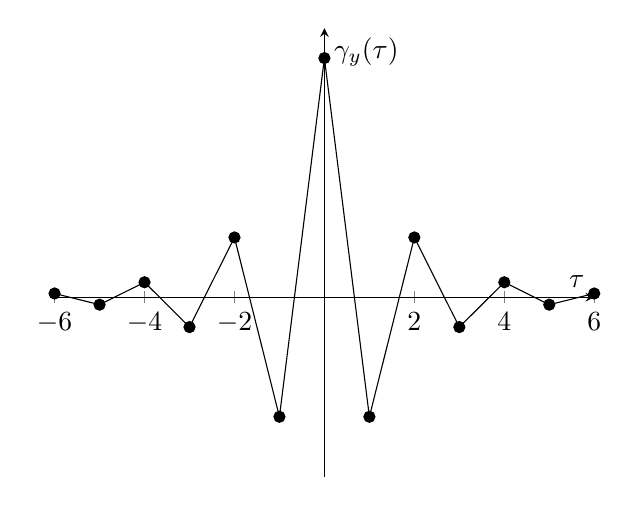
\begin{tikzpicture}

		\begin{axis}
		[
			axis x line=middle,
			axis y line=middle,
			ytick = \empty,
			xlabel={$\tau$},
			ylabel={$\gamma_y(\tau)$},
			xmin=-6, xmax=6,
			ymin=-1, ymax=1.5,
		]
		\addplot+[domain=-6:6, samples at={-6,...,6},color=black,mark options={
		fill=black}]{(-0.5)^abs(x)/(1-(-0.5)^2)};
		\end{axis}

		\end{tikzpicture}}
		\caption{Case $-1<a<0$.}
	\end{subfigure}
	\caption{Graphical representation of the covariance function for AR($1$) processes.}
\end{figure}
\FloatBarrier

\subsection{ARMA processes}
Let us consider the ARMA($m,n$) process generated according to:
\begin{align*}
	y(t) & = a_{1} y(t-1)+\cdots+a_{m} y(t-m)\\
	     &\quad +c_{0} e(t)+\cdots+c_{n} e(t-n) \quad \text{where} \quad e(t) \sim \WN(0, \lambda^{2})
\end{align*}


\textbf{Mean.}
\begin{align*}
	\E[y(t)] &=\E\left[a_{1} y(t-1)+\cdots+a_{m} y(t-m)+c_{0} e(t)+\cdots+c_{n} e(t-n)\right] \\
	&=a_{1} \E[y(t-1)]+\cdots+a_{m} \E[y(t-m)]+c_{0} \E[e(t)]+\cdots+c_{n} \E[e(t-n)]
\end{align*}
$$
m_{y}=a_{1} m_{y}+\cdots+a_{m} m_{y}+c_{0} \cdot 0+\cdots+c_{n} \cdot 0
$$

By asymptotic stability we can prove\footnote{It will not be done in this text.} that $(1-a_1-\cdots-a_m)\neq 0$, i.e. $m_{y}=0$.

\textbf{Covariance.}
\begin{align*}
	\gamma_{y}(0) = \E[y(t)^{2}] &= \E\left[\left(a_{1} y(t-1) + \cdots + a_{m} y(t-m) + c_{0} e(t) + \cdots + c_{n} e(t-n)\right)^{2}\right]\\
	&= a_{1}^{2} \E[y(t-1)^{2}] + a_{2}^{2} \E[y(t-2)^{2}] + \cdots+a_{m}^{2} \E[y(t-m)^{2}]\\
	&\qquad + 2 a_{1} a_{2} \E[y(t-1) y(t-2)] + 2 a_{1} a_{3} \E[y(t-1) y(t-3)] + \cdots \\
	&\qquad + c_{0}^{2} \E[e(t)^{2}] + c_{1}^2 \E[e(t-1)^2] + \cdots+c_{n}^2 \E[e(t-n)^2]\\
	&\qquad + 2 a_{1} c_{0} \E[y(t-1) e(t)] + 2 a_{1} c_{1} \E[y(t-1) e(t-1)] + \cdots\\
	&= (a_{1}^{2} + a_{2}^{2} + \cdots+a_{m}^{2})\cdot\gamma_{y}(0)\\
	&\qquad + 2 a_{1} a_{2} \gamma_{y}(1) + 2 a_{1} a_{3} \gamma_{y}(2) + \cdots \\
	&\qquad + (c_{0}^{2} + c_{1}^2 + \cdots+c_{n}^2)\cdot\lambda^2\\
	&\qquad + 2 a_{1} c_{0} \E[y(t-1) e(t)] + 2 a_{1} c_{1} \E[y(t-1) e(t-1)] + \cdots\\
\end{align*}

Then
\[
	\gamma (1)=\E[y(t) y(t-1)] = \E\left[\left(a_{1} y(t-1)+\cdots+a_{m} y(t-m)+c_{0} e(t)+\cdots+c_{n} e(t-n)\right) y(t-1)\right]
\]
Proceeding this way we get $m$ variables and $m$ linear equations (\emph{Yule--Walker equations} for an ARMA process).

Then $\gamma_{y}(m), \gamma_{y}(m+1), \ldots$ can be recursively computed from $\gamma_{y}(0), \gamma_{y}(1), \ldots, \gamma_{y}(m-1)$.